% Copyright (c) 2003-2021 Robert Ryszard Paciorek <rrp@opcode.eu.org>
% 
% MIT License
% 
% Permission is hereby granted, free of charge, to any person obtaining a copy
% of this software and associated documentation files (the "Software"), to deal
% in the Software without restriction, including without limitation the rights
% to use, copy, modify, merge, publish, distribute, sublicense, and/or sell
% copies of the Software, and to permit persons to whom the Software is
% furnished to do so, subject to the following conditions:
% 
% The above copyright notice and this permission notice shall be included in all
% copies or substantial portions of the Software.
% 
% THE SOFTWARE IS PROVIDED "AS IS", WITHOUT WARRANTY OF ANY KIND, EXPRESS OR
% IMPLIED, INCLUDING BUT NOT LIMITED TO THE WARRANTIES OF MERCHANTABILITY,
% FITNESS FOR A PARTICULAR PURPOSE AND NONINFRINGEMENT. IN NO EVENT SHALL THE
% AUTHORS OR COPYRIGHT HOLDERS BE LIABLE FOR ANY CLAIM, DAMAGES OR OTHER
% LIABILITY, WHETHER IN AN ACTION OF CONTRACT, TORT OR OTHERWISE, ARISING FROM,
% OUT OF OR IN CONNECTION WITH THE SOFTWARE OR THE USE OR OTHER DEALINGS IN THE
% SOFTWARE.

\documentclass{pdfBooklets}

\title{Elektronika (trochę) bardziej zaawansowana}
\author{%
	Robert Ryszard Paciorek\\\normalsize\ttfamily <rrp@opcode.eu.org>
}
\date  {2021-08-07}

\makeatletter\hypersetup{
	pdftitle = {\@title}, pdfauthor = {\@author}
}\makeatother

\newcommand\minifrac[2]{%
	\raisebox{.3ex}{$#1$}/\raisebox{-.6ex}{$#2$}
}
\newcommand\inpoint[1]{%
	\hspace{.4ex}\raisebox{-.55ex}{\scalebox{0.7}{$\bigg|_{#1}$}}\hspace{-.8ex}
}

\newcommand\verbhref[2]{\href{#1}{#2}\footnote{\url{#1}}}

\begin{document}

\maketitle

\section{Wprowadzenie}

Dokument omawia trochę bardziej zaawansowane tematy elektroniczne, głównie związane z układami opartymi na tranzystorach bipolarnych.
Zagadnienia związane z podstawami elektroniki, podstawowymi elementami elektronicznymi oraz podstawą działania tranzystorów omówione są w \textit{\verbhref{http://www.opcode.eu.org/Wprowadzenie_do_elektroniki.pdf}{Wprowadzenie do elektroniki}}.
Zagadnienia związane z prądem przemiennym, impedancją omówione są w \textit{\verbhref{http://www.opcode.eu.org/Podstawy_elektryki.pdf}{Podstawy „elektryki”}}.
Rekomendujemy wcześniejsze zapoznanie się z tymi tematami.

\section{Obwody prądu zmiennego}
Celem łatwiejszego obliczania obwodów prądu zmiennego możemy rozdzielać je na część dla prądu stałego (DC) i zmiennego (AC).
Dla prądu stałego: źródło napięcia zmiennego i cewka jest zwarciem, kondensator jest przerwą w obwodzie.
Dla prądu zmiennego: źródło napięcia stałego jest zwarciem, źródło prądu stałego jest rozwarciem, kondensator (jeżeli ma bardzo dużą / „nieskończoną” pojemność) jest zwarciem.
Należy szczególną uwagę zwrócić na powstające po zastosowaniu takich trików łączenia elementów - często łączenia wyglądające na szeregowe są łączeniami równoległymi.
Należy także pamiętać o powstającej „drugiej gałęzi” prowadzącej również do masy.

Stałą czasową $\tau = RC$ wyznacza pojemność kondensatora i jego oporowe otoczenie
	(rezystory które „widzi” kondensator i to w jaki sposób je „widzi” - w szczególności rezystory położone po obu stronach kondensatora mogą być połączone szeregowo poprzez masę).
$1/\tau$ odpowiada dolnej lub górnej (zależnie od układu) częstotliwości granicznej filtra górno lub dolno przepustowego.
Należy mieć świadomość że dla prądu stałego każdy (sprawny) kondensator zachowuje się jak rozwarcie oraz że dla odpowiednio dużych częstości
	(zależnych od pojemności kondensatora - im większa tym niższe te częstotliwości) kondensator przewodzi prąd zmienny praktycznie bez strat.

\subsection{Cewka i kondensator}
Kondensator gromadzi ładunek (napięcie), natomiast cewka potrafi magazynować prąd (po odłączeniu zasilania che ona wyrzucić z siebie prąd a nie ma na sobie jakiś ładunek).
Dlatego należy uważać na przebicia w układach kluczujących cewkę.
$$\rm{pojemność:}\qquad\Delta T={C \cdot \Delta U \over I}$$
$$\rm{indukcyjność:}\qquad\Delta T={L \cdot \Delta I \over U}$$
Wyróżnia się przede wszystkim cewki: powietrzne, na rdzeniu żelaznym i na rdzeniu ferrytowym. Ferryt bardzo silnie zwiększa indukcyjność cewki, ale ogranicza od góry częstotliwość pracy cewki. Ponadto przy odpowiednio dużym prądzie może dochodzić do nasycenia rdzenia, które objawia się tym że zaczyna in hamować wzrost pola zamiast go poprawiać.

\subsection{Metoda superpozycji}
Pozwala ona na rozdzielenie obwodu zawierającego kilka źródeł prądu i napięcia.
Obwód rozkładamy na tyle przypadków ile mamy źródeł niezależnych, w każdym z nich pozostawiamy tylko jedno (inne) źródło niezależne.
Pozostałe źródła zastępujemy zwarciem (źródła napięciowe) albo rozwarciem - źródła prądowe (z punktu widzenia źródła prądowego źródło napięcia jest zwarciem - punkt potencjału V jest równoprawny punktowi potencjału masy).
W każdym obwodzie znajdujemy składową (pochodzącą od niepominiętego źródła) szukanego prądu lub napięcia. 
Należy też zwrócić uwagę na kierunki napięć (ich znak) - prąd wypływający z rezystancji oznacza ujemne napięcie na tejże.
Całkowity szukany prąd lub napięcie jest sumą składowych.

\section{Źródła prądowe i napięciowe}
Na idealnym źródle prądowym może odłożyć się dowolne napięcie i zawsze płynie przez nie prąd ustalony przez wartość tego źródła. Przez idealne źródło napięcia można przepuścić dowolny prąd i zawsze napięcie pomiędzy jego zaciskami pozostaje stałe i określone wartością źródła.

\subsection{Zasada Thevenena i Zasada Nortona}
Pierwsza z nich mówi iż dowolny układ źródeł i oporów liniowych może być zastąpiony pojedynczym idealnym źródłem napięciowym (o napięciu równym napięciu na zastępowanym układzie gdy jest rozwarty - nie wpływa, ani nie wypływa z niego prąd) połączonym szeregowo z rezystancją zastępczą (obliczana po zastąpieniu wszystkich źródeł napięciowych zwarciami, a prądowych rozwarciami).
Druga mówi o możliwości zastąpienia takiego układu idealnym źródłem prądowym (o wartości prądu obliczanej przy zwartych zaciskach zastępowanego układu) z dołączoną równolegle rezystancją (obliczaną tak jak w poprzednim przypadku).


\section{Złącze PN - dioda}
\href{https://pl.wikipedia.org/wiki/Dioda półprzewodnikowa}{Dioda półprzewodnikowa} to w istocie pojedyncze \href{https://pl.wikipedia.org/wiki/Złącze p-n}{złącze p-n}.
Niespolaryzowane złącze odpowiada sytuacji pokazanej na poniższym rysunku (kolor zielony).
W takim wypadku prąd rekombinacji równoważony jest poprzez prąd generacji.

\begin{center}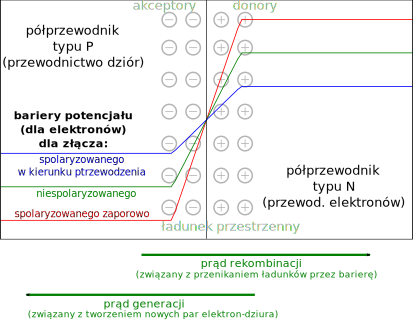
\includegraphics{img/elektronika2/zlacze_pn}\end{center}

Polaryzacja w kierunku przewodzenia (gdy $U_P > U_N$) powoduje obniżenie bariery potencjału (dokładniej to obu barier - pokazanej na rysunku bariery dla elektronów oraz analogicznej bariery dla dziur).
Efektem tego jest wzrost prądu rekombinacji, co przy niezmienionym prądzie generacji (zależy on od złącza a nie od bariery potencjału), prowadzi do powstania wypadkowego prądu płynącego przez złącze.

Typową eksponencjalną charakterystykę $I_F(U_F)$ złącza PN można przedstawić wzorem $$I_F = I_S \exp(U_F/\varphi_{_T} -1)$$ gdzie $\varphi_{_T} = kT/e$ i typowo wynosi około 25mV, natomiast $I_S$ zależne jest od typu złącza i konkretnego egzemplarza.
Dzięki temu możemy zapisać rezystancję dynamiczną diody (związaną z spadkiem napięcia na przewodzącym złączu) jako $r_D = \varphi_{_T}/I_{FQ}$.
Tą cechę diody można wykorzystać np. do stworzenia regulowanego dzielnika (regulowane źródło prądu DC + dioda) będącego w stanie zmniejszać amplitudę sygnałów dużej częstości (gdzie nie możemy zastosować potencjometru, gdyż za bardzo zagłuszyłby sygnał).

\section{Tranzystor}

\href{https://pl.wikipedia.org/wiki/Tranzystor}{Tranzystor} jest to element o regulowanym elektronicznie oporze (tak na prawdę regulowany jest przepływający prąd), często wykorzystywany do wzmacniania sygnałów lub jako przełącznik elektroniczny.

\href{https://pl.wikipedia.org/wiki/Tranzystor bipolarny}{Tranzystor bipolarny} posiada trzy wyprowadzenia - emiter (E), baza (B), kolektor (C), przepływający przez niego prąd reguluje się poprzez przyłożenie napięcia między bazą a emiterem. W  tranzystorach PNP prąd płynie od emitera (o wyższym potencjale) do kolektora, w NPN na odwrót. Należy też pamiętać że tranzystor bipolarny to nie bramka logiczna czy coś w tym stylu - jeżeli przyłożymy napięcie w kierunku przewodzenia do bramki to prąd popłynie nawet gdy nie ma przyłożonego napięcia kolektor - emiter (bramka nie jest izolowana).

Przy wzmacnianiu sygnałów tranzystor pracuje w \href{https://pl.wikipedia.org/wiki/Tranzystor bipolarny#Stany_pracy}{stanie aktywnym} czyli napięcie przyłożone do bazy jest pomiędzy napięciem kolektora a emitera. W przypadku wykorzystywania jako przełącznik tranzystor pracuje w stanach zatkania (nie przewodzi) lub nasycenia (nie ogranicza). Poniższa ilustracja przedstawia podstawową polaryzację tranzystora.

\begin{center}\includegraphics{img/elektronika2/tranzystory}\end{center}

Strzałka w symbolu tranzystora (umieszczana na emiterze) pokazuje kierunek przepływu prądu przez emiter.
Pokazuje ona kierunek przepływu prądu przez złącz P-N (diodę) baza-emiter, zatem wskazuje także kierunek prądu bazy.

W stanie aktywnym prąd kolektora jest regulowany poprzez napięcie baza-emiter.
Zatem na tranzystor możemy patrzeć jak na diodę w której rozdzieliliśmy styk odpowiedzialny za przyłożone napięcie od styku którym płynie prąd - tak jak w diodzie {\bf prąd zależy wykładniczo od przyłożonego napięcia}, tyle że napięcie przykładamy pomiędzy E i B, a prąd płynie głównie pomiędzy E i C (jest także przepływ pomiędzy B i E związany z rekombinacją elektronów w bazie i wstrzykiwaniem ładunków baza-emiter - ze względu na różnice w domieszkowaniu słabszym niż wstrzykiwanie emiter-baza).
Zatem prąd płynący przez tranzystor (prąd kolektora) zależy tylko od napięcia diody baza-emiter.

Ciekawym przypadkiem jest wymuszone $I_c = 0$ (gdy kontakt kolektora pozostaje niepodłączony) - wtedy prąd bazy musi wzrosnąć do takiej wartości aby zrównoważyć prąd emitera (on nie ulega zmianie gdyż zależy tylko od napięcia baza-emiter), natomiast na złączu kolektorowym będzie 0.5V (trochę mniej niż spadek na diodzie gdyż kolektor jest słabo domieszkowany).

Możliwe jest także {\bf sterowanie tranzystora prądem bazy, a nie napięciem BE}.
W takim wypadku napięcie pomiędzy bazą a emiterem wynosi około 0.6V - 0.7V (warto pamiętać o tym napięciu przy obliczaniu rezystancji wymaganej aby uzyskać pożądany prąd bazy).
W wypadku tym do bazy wprowadzamy dodatkowe ładunki (w NPN są to dziury), co owocuje wciąganiem w ten obszar ładunków przeciwnych z emitera.
Większość z nich jednak nie zdąży zrekombinować w bazie (jest ona cienka) tylko przeleci do kolektora, którego prąd dany jest zależnością: $I_C = \beta I_B$, gdzie $\beta$ to wzmocnienie tranzystora.
Zatem tranzystor zachowuje się jak (regulowane prądem) źródło prądowe.
W obwodzie kolektora wprowadza się zazwyczaj rezystor (Rc) mający na celu zamianę sygnału prądowego uzyskiwanego dzięki tranzystorowi na napięcie, z którego jest łatwiej korzystać niż z prądu.

\begin{center}\includegraphics{img/elektronika2/uklady_polaryzacji_npn}\end{center}

Ze względu na znaczny rozrzut wartości $\beta$ pomiędzy egzemplarzami układ taki jest trudny do praktycznego stosowania (rezystor ustalający prąd bazy należałoby dobierać do konkretnego tranzystora / stosować rezystor regulowany i go dostrajać), dlatego najczęściej stosowany jest „{\bf układ z stałym potencjałem bazy}”.
W układzie takim do bazy podłączamy pewien ustalony potencjał (na tle wysoki aby nieznajomość spadku na złączu PN - czy to jest 0.6V czy 0.7V itp - była pomijalna), a poprzez zastosowanie opornika emiterowego (Re) ustalamy prąd emitera.
Na jego wartość nie ma wpływu to co dzieje się w kolektorze, gdyż zależy on tylko od napięcia baza-emiter (w przypadku niepodłączonego kolektora całość prądu emitera płynie przez bazę, w przeciwnym razie przez bazę płynie $I_B = \frac{I_E}{\beta + 1}$).
Dzięki takiemu zabiegowi (ustaleniu prądu emitera) udało się bardzo skutecznie zminimalizować wpływ wartości $\beta$ na prąd kolektora gdyż $I_C = I_E - I_B = I_E \frac{\beta}{\beta+1}$, a jako że $\beta \gg 1$ to $I_C \approx I_E$.

W układzie z stałym potencjałem bazy jeżeli spadek na rezystancji wewnętrznej źródła, którym jest dzielnik R1 R2, jest istotny (w porównaniu z nieznajomością spadku napięcia na złączu baza-emiter) należy uwzględniać tą rezystancję w obliczaniu prądu emitera: $E_z - I_E\frac{1}{\beta + 1}R_z - U_{BEP} - I_ER_E = 0$.
Warto wspomnieć iż za polaryzację bazy może być odpowiedzialne inne źródło napięcia niż klasyczny dzielnik (np. dzielnik z diodą Zenera).

% NPN przewodzi gdy napięcie miedzy bramką (B) a emiterem (E) przekroczy określoną wartość - około 0.6V (gdy zerowe lub ujemne to stan zatkania)

%zatkania (nie przewodzi) - napięcie bazy równe lub mniejsze (NPN) od napięcia emitera
%nasycenia (nie ogranicza) - napięcie bazy równe lub większe (NPN) od napięcia kolektora.

Stan nasycenia polega na polaryzacji obu złącz w stanie przewodzenia (na typie P napięcie wyższe o około 0.6V niż na typie N).
Na tranzystorze w stanie nasycenia występuje spadek napięcia $U_{CE} = U_{BE} - U_{BC} \approx 0.7 - 0.5 = 0.2\rm{V}$.
Jeżeli spadek ten może być przeszkodą należy rozważyć zastosowanie trybu nasyconego inwersyjnego zamieniony kolektor z emiterem), gdzie on jest dużo bardziej bliski zeru.
Tranzystor wchodzi w ten stan gdy $V_E < V_B > V_C$ (NPN) lub $V_E > V_B < V_C$ (PNP).
W przypadku regulacji prądem bazy ma to miejsce gdy $I_C = \beta I_B > I_{C_{max\ ukl}}$ (czyli gdy spadek na obciążeniu wynikły z obliczonego prądu kolektora spowodowałby odłożenie na nim napięcia większego niż napięcie zasilania).
Tranzystor w stan nasycenia wprowadzać należy z (dwu - trzy krotnym) zapasem prądu nasycającego, czyli $R_B << {U_{Ster}-U_{BE} \over I_B}$.

Stan zatkania polega na zaporowej polaryzacji obu złącz czyli $V_E \geq V_B \leq V_C$ (NPN) lub $V_E \leq V_B \geq V_C$ (PNP).
W tym wypadku należy szczególnie zwrócić uwagę na (niewielkie) napięcia przebicia spolaryzowanego zaporowo złącza baza-emiter).

\begin{center}\includegraphics{img/elektronika2/nasycenie-zatkanie}\end{center}

Nasycenie NPN gdy: $I_C > V_{cc} / R_{L_{min}}$, gdzie $I_C = \beta_{min} I_B$, a $I_B = \frac{V_{ster} - 0.7V}{R_B}$ zatem otrzymaliśmy warunek na rezystor bazy: $R_B < \beta_{min} (V_{ster} - 0.7V) \frac{R_{L_{min}}}{V_{cc}}$. Dla PNP rozumujemy analogicznie, tyle że prąd bazy zależy od napięcia zasilania a nie sterowania, czyli: $R_B < \beta_{min} (V_{cc} - 0.7V) \frac{R_{L_{min}}}{V_{cc}}$. Warto zauważyć, że $\frac{R_{L_{min}}}{V_{cc}} = 1/I_{C_{max\ ukl}}$.

\subsection{JFET}
\href{https://pl.wikipedia.org/wiki/Tranzystor polowy}{Tranzystor unipolarny} (polowy) posiada trzy wyprowadzenia - dren (D), bramka (G), źródło (S), regulacja odbywa się poprzez regulację napięcia między źródłem a bramką. W tranzystorach tych sterowanie odbywa się polem elektrycznym (z tąd nazwa polowy), a prąd bramki (gdy tranzystor jest dobrze spolaryzowany) jest pomijalnie mały. Dzięki temu mogą służyć do uzyskania wejścia o dużej rezystancji wejściowej.

Dostępne na rynku tranzystory \href{https://pl.wikipedia.org/wiki/Tranzystor polowy złączowy}{JFET} z kanałem N steruje się poprzez ujemną polaryzację bramki wobec źródła. W przypadku gdy potencjał bramki jest odpowiednio ujemny (mniejszy od charakterystycznego - w zasadzie dla danego egzemplarza - napięcia „odcięcia” $U_{GS_{off}} = U_T$) tranzystor nie przewodzi (prąd DS pomijalne mały). W przeciwnym wypadku w zależności od przyłożonego napięcia DS tranzystor ten zachowuje się jak regulowane źródło prądowe (gdy to napięcie większe od różnicy pomiędzy obecnym napięciem GS a napięciem odcięcia) lub regulowany rezystor (gdy mniejsze). Maksymalny dla danego napięcia prąd (oznaczany $I_{DSS}$) płynie gdy napięcie pomiędzy bramką a źródłem jest równe zero (w zasadzie troszkę większe od zera, ale tak aby nie spolaryzować złącza w stan przewodzenia).

Niestety tranzystory te cechują się dużym rozrzutem kluczowych parametrów (napięcie GS przy którym następuje zatkanie oraz maksymalny prąd przewodzenia) pomiędzy egzemplarzami. Najprostszym przykładem zastosowania jest źródło prądowe utworzone poprzez podłączenie bramki do masy oraz źródła poprzez (regulowany) opornik do masy. Tranzystor ten w stanie z otwartym złączem kanał-bramka może być wykorzystany jako dioda mało upływowa.

$$I_D = \left\{\begin{array}{ll}
	0
		&  U_{GS} < U_T\\
	\beta \cdot (U_{GS}-U_T)^2
		&  U_{GS} \geq U_T \wedge U_{DS} > U_{GS} - U_T\\
	\beta \cdot U_{GS} \cdot [2(U_{GS}-U_T) - U_{DS}]
		&  U_{GS} \geq U_T \wedge U_{DS} \leq  U_{GS} - U_T \wedge U_{DS} \geq 0
\end{array}\right. \rm{,\ gdzie\ } \beta = {I_{DSS} \over {U_T}^2}$$

Tranzystory J-FET cechują się symetrią pomiędzy źródłem a drenem, ale przy projektowaniu układów z nimi warto wiedzieć którą elektrodę traktujemy w jaki sposób.
Tranzystory J-FET zazwyczaj polaryzuje się poprzez połączenie przez duży opór ($R_B$ rzędu giga omów) bramki do masy, co wraz z małym prądem bramki zapewnia na niej potencjał 0V.
Jako że J-FET przy $U_{GS} = 0$ przewodzi (i to maksymalny prąd) to taka polaryzacja powoduje przepływ prądu DS co w związku z oporem $R_S$ pomiędzy źródłem a masą prowadzi do podniesienia potencjału na źródle czyli pojawienia się ujemnego napięcia $U_{GS} = U_{R_S}$ i ograniczenia prądu.

\begin{center}\includegraphics{img/elektronika2/jfet}\end{center}

Jako że występują dwa tryby pracy JFETów to przy wykonywaniu obliczeń konieczna jest identyfikacja z którym trybem pracy mamy do czynienia.
Możemy wykonać to orientacyjnie na podstawie porównania wartości $R_D$ i $R_S$ - gdy $R_D >> R_0$ to możemy podejrzewać obszar triodowy / nienasycenia ($I_D = \beta \cdot U_{GS} \cdot [2(U_{GS}-U_T) - U_{DS}]$), gdzie tranzystor zachowuje się jak opornik regulowany.
Jeżeli jednak nie zgodzą nam się znaki napięć musimy policzyć dla obszaru pentodowego / nasycenia ($I_D = \beta \cdot (U_{GS}-U_T)^2$). Warto także pamiętać że $I_D = {|U_{GS}| \over R_S}$

\section{Tyrystor, triak}
\href{https://pl.wikipedia.org/wiki/Tyrystor}{Tyrystor} jest to element o regulowanym elektrycznie stanie przewodzenia, przewodzić on może od anody do katody (tylko w tą stronę), pod warunkiem że zostanie wyzwolony impulsem bramki (dodatnie napięcie względem katody) bądź wzrostem napięcia przyłożonego.
W odróżnieniu od tranzystora tyrystor przewodzi również po zaniku napięcia przyłożonego do bramki (przerywa dopiero gdy zostanie przerwane przewodzenie).
\href{https://pl.wikipedia.org/wiki/Triak}{Triak} jest w zasadzie dwukierunkową wersją tyrystora odpowiadającą funkcjonalnie połączonym antyrównolegle dwóm tyrystorm.

W zrozumieniu jak to działa przydany może być schemat zastępczy tyrystora na tranzystorach bipolarnych:

\begin{center}\includegraphics{img/elektronika2/tyrystor}\end{center}


\section{Radiatory}

Często elementy elektroniczne wymagają dodatkowego chłodzenia - przynajmniej w postaci radiatora.
Jego dobór przeprowadza się w oparciu o wymaganą \href{https://pl.wikipedia.org/wiki/Rezystancja_termiczna}{rezystanjcę termiczną}:
%
$$R_{th (radiator)} = \frac{T_{max} - T_{amb}}{P} - (R_{th (zlacze-obudowa)} + R_{th (obudowa-radiator)})$$
%
Gdzie:
\begin{itemize}
	\item $T_{max}$ – maksymalna temperatura układu
	\item $R_{th (zlacze-obudowa)}$ – rezystancja termiczna złącze-obudowa
\end{itemize}
to dane katalogowe chłodzonego układu (tranzystora, triaka, ...).
Natomiast jako $R_{th (obudowa-radiator)}$ (rezystancja termiczna obudowa-radiator), przyjmuje się wartość od 1K/W (bezpośrednie przykręcenie) do 0.2K/W (pasta silikonowa).

Zobacz także \href{http://www.elportal.pl/pdf/k01/32_13.pdf}{artykuł na ten temat w EdW}.

\subsection{przykład}

Dla BTA16, temperatury otoczenia 50 stopni C i 10 W strat (co odpowiada przepuszczaniu przez triaka 10A) mamy:
%
$$R_{th (radiator)} = \frac{125-50}{10} - (2.1 + 0.2) = 5.4 \rm{K/W}$$
%
czyli wartość rezystancji termicznej radiatora musi być \strong{mniejsza} lub równa od 5.4K/W.

\section{Układy tranzystorowe}

\begin{ProTip}{Rezystancja wejściowa/wyjściowa układu}
Jest to wartość niezależna od prądu wejściowego (prądu pobieranego zawsze przez dany układ) i zdefiniować możemy ją jako iloczyn przyrostu napięcia do przyrostu prądu.
\end{ProTip}

\subsection{Wzmacniacz małych sygnałów}

Typowym zastosowaniem tranzystora jest wzmacnianie sygnałów.
Dalej będziemy przez jakiś czas przyjmować że mamy doczynienia z „małym sygnałem” czyli takim którego dołożenie powoduje niewielkie odchylenia od punktu pracy (takie że można zaniedbać krzywiznę charakterystyki).
Wyróżnić można 3 podstawowe układy pracy tranzystora bipolarnego w wzmacniaczu sygnału (pokazane na przykładzie układu polaryzacji z opornikiem emiterowym):

\begin{center}\includegraphics{img/elektronika2/uklady_pracy_npn}\end{center}

W przypadku pracy w układzie wspólnego emitera, generator sygnału dokładamy poprzez kondensator do spolaryzowanej w stanie aktywnym bazy.
W efekcie tego na stały prąd wyjściowy nakłada się prąd związany z sygnałem wejściowym wynoszący $I_C \inpoint{AC} = g_m U_{b'e} \inpoint{AC}$, gdzie $g_m = {I_{CQ} \over \varphi_{_T}} \approx {1 \over r_{eb'}}$ jest nachyleniem charakterystyki w punkcie pracy, a $U_{b'e} \inpoint{AC}$ jest sygnałem dołożonym na złącze baza-emiter (w przybliżeniu równym sygnałowi wejściowemu).

W prezentowanej sytuacji (układ z opornikiem emiterowym) przy rozważaniu mechanizmu tego procesu lepiej byłoby rozumować właśnie poprzez rezystancję dynamiczną emitera $r_{eb'}$ (a nie $g_m$, które jest właściwe dla polaryzacji stałym prądem bazy), gdyż w układzie takim zmiana napięcia zasilającego przekłada się w niezmiennym stosunku (określonym głównie przez wartość oporu emiterowego) na prąd emitera, a ten jest w przybliżeniu równy prądowi kolektora.
Zatem uzyskanie wzmocnienia innego niż 1 wymaga zwarcia emitera dla sygnałów zmiennych do masy (kondensator CE) i wtedy właśnie opór dynamiczny $r_{eb'}$ powoduje że uzyskujemy skończone wzmocnienie.

Każdy wzmacniacz charakteryzuje się następującymi parametrami (podane sposoby obliczania dla układu pracy wspólny emiter):\begin{itemize}
	\item rezystancja wejściowa - utworzona przez rezystancję zastępczą oporników ustalających punkt pracy oraz oporu dynamicznego złącza PN pomiędzy bazą a emiterem wynoszącą: $r_{b'e}=\beta r_{eb'} = \beta \frac{\varphi_{_T}}{I_E} \approx \beta \frac{\varphi_{_T}}{I_C}$
	\item rezystancja wyjściowa - utworzona przez rezystor łączący kolektor z zasilaniem
	\item wzmocnienie napięciowe zwykłe $|k_u| = U_{wy} / U_{we} = g_m R_C$ (niekiedy umawiamy się że obejmuje też rezystancję obciążenia a nie tylko $R_C$)
	\item wzmocnienie napięciowe skuteczne (czyli uwzględniające rezystancję wewnętrzną źródła sygnału) $|k_{us}| = k_u \frac{R_{we}}{R_{we} + R_G}$
\end{itemize}

\subsubsection{obliczanie układu typu wspólny emiter}

\paragraph{Ustalanie punktu pracy (bipolarny, stały prąd bazy):}
\begin{enumerate}
	\item $I_B = I_{CQ} / \beta$
	\item $R_B = {U_{CC} - U_{BE} \over I_B}$
	\item $R_C = {U_{CC} - U_{CEQ} \over I_{CQ}}$
	\item rozrzut $\beta$ załatwiamy licząc dla średniej i sprawdzając czy dla maksymalnej nie prowadzi do nasycenia
\end{enumerate}

\paragraph{Obliczenie punktu pracy i parametrów układu (bipolarny, stały prąd bazy):}
\begin{enumerate}
	\item $U_{RB} = U_{CC} - U_{BE}$
	\item $I_B = {U_{RB} \over  R_B}$
	\item {\bf $I_C = \beta I_B$}
	\item {\bf $U_{CE} = U_{CC} - R_C I_C$}
	\item $R_{WE} = R_B || r_{b'e}$
	\item $R_{WY} = R_C$
	\item $k_{u} = {U_{WY} \over U_{WE}} = g_m (R_C || R_O) = \frac{I_C}{\varphi_{_T}} \frac{R_C R_O}{R_C + R_O}$
	\item $k_{us} = k_u \frac{R_{WE}}{R_{WE} + R_G}$
	\item $k_{i} =  k_{u} \frac{R_{WE}}{R_{0}}$
	\item $k_{is} = \frac{I_O}{I_G} = \frac{U_O/R_O}{U_G/R_G} = k_{uS} \frac{R_{G}}{R_{0}}$
	\item $k_{ps} = 4 k_{is} k_{us}$
\end{enumerate}

\paragraph{Ustalanie punktu pracy (bipolarny, opornik emiterowy):}
\begin{enumerate}
	\item przyjmujemy założenie o spadku napięcia na $U_{RE}$
	\item $R_E = {U_{RE} \over I_{CQ}}$
	\item $U_{RC} = U_{CC} - U_{CEQ} - U_{RE}$
	\item $R_C = {U_{RC} \over I_{CQ}}$
	\item dzielnik - napięcie wyjściowe $U_B = U_{RE} + U_{BE}$
	\item obliczamy dla sztywnego dzielnika (spadek napięcia wyjściowego związany z prądem bazy < 0.1V)
	\item weryfikacja dzielnika - obliczenie $U_{BE}$ z $E_{BZ} = I_B R_{BZ} + U_{BE} + I_E R_E$, gdzie $E_{BZ} = U_{CC}\frac{R_{B2}}{R_{B1} + R_{B2}} \approx 2.7\rm{V}$
	\item warto sprawdzić także czy dzielnik nie jest zbyt sztywny (nie wybija sygnału)
\end{enumerate}

\paragraph{Obliczenie punktu pracy i parametrów układu (bipolarny, opornik emiterowy):}
\begin{enumerate}
	\item $R_{BZ} = R_{B1} || R_{B2}$
	\item $E_{BZ} = U_{CC}\frac{R_{B2}}{R_{B1} + R_{B2}}$
	\item $U_{RE} = E_{BZ} - U_{BE}$ (zakładamy tutaj sztywny dzielnik - spadek na $R_{BZ}$ pomijalnie mały)
	\item {\bf $I_C \approx I_E = {U_{RE} \over R_E}$}
	\item znając $I_B = {I_E \over \beta +1}$ weryfikujemy założenie o sztywności dzielnika licząc spadek napięcia na $R_{BZ}$ --- $U_{RBZ} = R_{BZ} I_B$
	\item $U_C = U_{CC} - U_{RC}$
	\item {\bf $U_{CE} = U_C - U_E$}
	\item $R_{WE} = R_{BZ} || (r_{b'e} + \beta R_E)$ lub $R_{WE} = R_{BZ} || r_{b'e}$ (gdy mamy $C_E$)
	\item pozostałe parametry ($R_{WY}$, $k_{u}$, $k_{us}$, $k_{i}$, $k_{is}$, $k_{ps}$) obliczamy tak samo jak przy „stałym prądzie bazy"
\end{enumerate}

Przy obliczaniu pojemności uwzględniamy ich otoczenie rezystorowe - $R_{WE} + R_G$ dla kondensatora wejściowego, $R_{WY} + R_O$ dla kondensatora wyjściowego oraz $R_E || \left(\frac{R_G||R_{BZ}}{\beta_{AC} + 1} + r_{eb'} \right)$ dla kondensatora emiterowego.

\paragraph{Ustalanie punktu pracy i parametrów układu (JFET):}
\begin{enumerate}
	\item $\beta = {I_{DSS} \over U_T^2}$
	\item obliczamy $U_{GS}$ w oparciu o zależności: $\beta (U_{GS} - U_T)^2 = - U_{GS} / R_S$ (przyjmujemy założenie o zakresie pentodowym)
	\item $I_D = - U_{GS} / R_S$
	\item $U_{RD} = I_D R_D$
	\item $U_{RS} = I_D R_S$
	\item $U_{DS} = V_{DD} - U_{RD} - U_{RS}$
	\item sprawdzamy czy zakres pentodowy - $U_{GS} \ge U_T$ i $U_{DS} \ge U_{GS} - U_T$
	\item $R_{WY} = R_D$
	\item $R_{WE} = R_B$
	\item $k_u = -g_m R_L$ (tak samo jak w bipolarnym, ale inne $g_m = {dI_D \over dU_{GS}}$ - dla zakresu pentodowego $g_m=2 \beta (U_{GS} - U_T)$)
	\item pozostałe parametry ($k_{us}$, $k_{i}$, $k_{is}$, $k_{ps}$) obliczamy w oparciu o powyższe $R_{WE}$, $R_{WY}$, $k_{u}$, tak samo jak przy bipolarnym
\end{enumerate}

\subsection{Wtórnik emiteorowy}
\begin{center}\includegraphics{img/elektronika2/wtornik}\end{center}

Każdy wtórnik jest układem typu „wspólny kolektor” (ale na odwrót nie zawsze).
Układ taki (w odróżnieniu od wspólnego emitera czy też wspólnej bazy) jest w stanie wzmacniać nie tylko małe ale także duże sygnały.
Jednak potrafi on wzmacniać tylko prąd - napięcie wyjściowe jest niemalże równe napięciu wejściowemu (dokładniej jest pomniejszone o spadek na aktywnym złączu PN).

Często wykorzystywany jest układ wtórnika z tzw. „sprzężeniem stałoprądowym” (bez odcinania składowej stałej na wejściu) i podwójnym (dodatnim i ujemnym) zasilaniem (służącym do ustalenia punktu pracy zamiast dzielnika podłączanego do bazy) przedstawiony na poniższej ilustracji.

Można spotkać się także z połączeniem dwóch tranzystorów pracujących w układzie w wtórnika.
W szczególności może być to J-FET z bipolarnym (aby uzyskać dużą rezystancję wejściową i małą wyjściową), lub tranzystory tego samego typu aby uzyskać większą wypadkową wartość $\beta$ (jest ona wtedy iloczynem wartości dla poszczególnych tranzystorów).

\subsubsection{obliczanie układu typu wtórnik emiterowy}
Punkt pracy ustalany tak samo jak dla układów WE.

\paragraph{Ustalanie parametrów układu (bipolarny):}
\begin{enumerate}
	\item $R_{WY} = R_E || {R_G + r_{b'e} \over \beta +1}$
	\item $R_{WE} = R_{b'e} + (\beta + 1) (R_E || R_L)$
	\item $k_u = {(\beta + 1) (R_E || R_L) \over R_{b'e} + (\beta + 1) (R_E || R_L)}$
\end{enumerate}

\paragraph{Ustalanie parametrów układu (JFET):}
\begin{enumerate}
	\item $R_{WY} = R_S || {1 \over g_m}$
	\item $R_{WE} = R_{B}$
	\item $k_u = {g_m (R_S || R_O) \over 1 + g_m (R_S || R_O)}$
\end{enumerate}


\subsection{Lustro prądowe}
\begin{center}\includegraphics{img/elektronika2/lustro}\end{center}

T1 i T2 muszą mieć zapewnioną tą samą temperaturę (najlepiej być wykonane w ramach jednego układu scalonego.
T1 pracuje jako dioda (stosujemy tranzystor aby zapewnić taką samą charakterystykę jak T2), która wraz z R1 tworzy sprzężony termicznie z T2 dzielnik sterujący tranzystorem T2. Układ ten sterowany prądem płynącym przez R1 powoduje przepływ (niemalże) takiego samego prądu poprzez RL.

\subsection{Wzmacniacz różnicowy}
\begin{center}\includegraphics{img/elektronika2/wzmacniacz_roznicowy}\end{center}

Układ ten może pełnić rolę klucza prądowego (gdy podany sygnał na tyle duży aby zatkać jeden z tranzystorów) lub wzmacniacza (gdy pracować będą oba tranzystory.
Układ jest czuły na różnicę napięć przyłożonych do in1 i in2.
Ree pełni rolę źródła prądowego (i powinien być tak dobrany wraz z -Vee aby zapewnić jego stabilność ...).

W przypadku układu z tranzystorami NPN „bardziej” przewodzić będzie tranzystor na wejściu którego jest większe napięcie (niż na tym drugim).
Fakt tego że on przewodzi powoduje ustalenie się potencjału w węźle łączącym emitery obu tranzystorów na wartość napięcia jego bazy pomniejszonego o spadek na przewodzącym złączu PN.
W sytuacji gdy napięcia baz obu tranzystorów są odpowiednio bliskie przewodzić będą oba, zakres ten określa się strefą przejściową i wynosi ona $4 \varphi_{_T}$.

%\begin{center}\includegraphics{img/elektronika2/wzmacniacz_roznicowy_przejsciowa}\end{center}

Jeżeli pracujemy w zakresie strefy przejściowej układ ten traktować należy jako wzmacniacz (poza tym zakresem jak wspomniano jest kluczem prądowym).
Posiada on wtedy wzmocnienie $k_{u_i} = \frac{R_{C_i}}{r_{eb'_1} + r_{eb'_2}}$, gdzie $i$ jest numerem wyjścia/rezystora kolektorowego z którego pobieramy napięcie wyjściowe.
Wzmocnienie wyjścia różnicowego jest sumą wzmocnień poszczególnych wyjść.
Wzmacniacz ten posiada także niestety wzmocnienie sumacyjne (wzmocnienie napięcia wchodzącego równocześnie na oba wejścia).
Wynika to z niemożności zastosowania idealnego źródła prądowego, a przy stosowaniu rzeczywistych zmiana napięcia na źródle (wynikła z z miany potencjału na emiterach) prowadzi do zmiany prądu płynącego przez źródło.

Jako że przy tranzystorach bipolarnych musimy umożliwić przepływ prądu bazy, a nawet przy MOSFETach musimy zapewnić polaryzację bramki określonym potencjałem, w przypadku wprowadzania na wejście sygnału z odcięciem składowej stałej (poprzez kondensator) musimy zastosować {\bf rezystory $R_B$} pomiędzy każdym z wejść a masą.
Oba te rezystory powinny mieć tą samą wartość, gdyż inna sytuacja byłaby równoważna dołożeniu na jedno z wejść jakiegoś stałego potencjału (innego niż dołożony do drugiego wejścia) a tego nie chcemy.
Podobnie gdy stosujemy sprzężenie stało-prądowe, a źródło sygnału ma znaczącą rezystancję wewnętrzną to do drugie wejście należy połączyć z masą przez taką samą rezystancję (rezystancje zastępcze widziane przez sygnał, podłączone do obu wejść powinny być jednakowe).

Często można się spotkać z modyfikacjami tego układu polegającymi na dołączaniu pomiędzy Ree a emiterami rezystorów celem powiększenia strefy przejściowej i jej linearyzacji.
Możliwe jest też także rozdzielenie gałęzi emiterowej na dwie i sprzężenie ich przy pomocy kondensatora - wtedy przenoszone są tylko sygnały zmienne (każdy z emiterów ma do polaryzacji swój własny Ree) dzięki czemu można układ ten realizować na tranzystorach dyskretnych.
Popularną modyfikacją tego układu jest dołączenie w miejsce RB1 i RB2 lustra prądowego przenoszącego prąd z gałęzi T1 (nie mamy wtedy wyjścia out1) na gałąź T2 (uzyskujemy wtedy dwukrotnie większe wzmocnienie na out2). Aby układ taki działał konieczne jest podłączenie rezystancji obciążenia do potencjału pomiędzy zasilaniem lustra a sumacyjnym napięciem wejściowym (składową będącą identyczną na obu wejściach).

\subsubsection{obliczanie punktu pracy, rezystancji i wzmocnień}
\begin{enumerate}
	\item $I_{CQ} = I_{EE}/2$ (także w niesymetrycznym!)
	\item $R_{WE} = 2 r_{b'e}$
	\item $R_{WY_i} = R_{C_i}$
	\item $k_{u_i} = {R_{C_i} \over r_{eb'_1} + r_{eb'_2}}$ (gdy korzystamy tylko z we1 to wy1 odwracające więc $k_{u_1}$ może być podawane jako ujemne)
	\item $k_{u_{sum}} = |k_{u_1}| +| k_{u_2}|$
\end{enumerate}
Ewentualna niesymetryczność wpływa na zakres napięć wyjściowych.

\subsection{Efekt Millera}
\href{https://pl.wikipedia.org/wiki/Efekt_Millera}{Efekt Millera} występuje w układach odwracających fazę i polega na tym iż impedancja widoczna z zewnątrz jest $k+1$ razy mniejsza (gdzie $k$ - wzmocnienie układu) niż rzeczywista impedancja pomiędzy wejściem a wyjściem.
Ponadto w tranzystorze występują pojemności pomiędzy bazą a emiterem oraz bazą a kolektorem.
A jedna z nich w układach odwracających fazę ulega efektowi Millera. To odgrywa on istotną rolę w ograniczeniu górnej częstotliwości układów wzmacniaczy.
$$C_{b'e} = \frac{1}{2 \pi r_{eb'} f_T} - C_{bk}$$
Podawany w katalogach parametr $f_T$ jest tylko wynikiem specyficznego pomiaru tej właśnie pojemności, a to jakie będzie związane z nią ograniczenie częstotliwości wynika z konkretnego układu w którym stosowany jest tranzystor.

\subsection{Boot Strap}
jest to efekt niejako przeciwny do efektu Millera - występuje on gdy mamy wzmocnienie napięciowe nie większe od jedności.
Pozwala ono na zmniejszanie impedancji włączonej równolegle z układem wzmacniającym (w przypadku wzmocnienia równego 1 impedancja taka znika całkowicie gdyż niejako obok niej wejście jest powielane na wyjście (napięcie na niej wynosi zero.
Może także robić za źródło prądowe gdy w szereg z wzmacniaczem mamy przesuwnik potencjału to na tej impedancji odkłada się stała różnica potencjałów, a zatem płynie stały prąd.

\subsection{Wzmacniacz operacyjny}
Jest to układ służący do wzmacniania bardzo wiele razy różnicy napięć wejściowych.
Na stopniu wejściowym posiada on wzmacniacz różnicowy z lustrem, dalej jest układ wzmacniający o dużym wzmocnieniu, a na stopniu wyjściowym wtórnik emiterowy.

Układ ten może być wykorzystywany jako komparator do porównywania napięć.
Ponadto komparatory scalone posiadają taki sam symbol, jednak są innymi układami - dużo szybciej przełączają swoje wyjście przy zmianie wejścia niż robi to wzmacniacz operacyjny.

\begin{center}\includegraphics{img/elektronika2/wzmacniacz_operacyjny}\end{center}

Jako iż wzmocnienie wzmacniaczy operacyjnych jest bardzo duże nie da się w praktyce wykorzystać ich bezpośrednio do wzmacniania sygnału.
Robi się to z wykorzystaniem sprzężenia zwrotnego, czyli podaniem przeskalowanego sygnału wyjściowego na wejście.
Dzięki temu że korzystamy z ujemnego sprzężenia układ zachowuje się stabilnie dążąc do utrzymania różnicy napięć wejściowych bliskiej zeru.
Wzmocnienie wzmacniacza odwracającego fazę wynosi $k_u = - {R_2 \over R_1}$, a wzmacniacza nie odwracającego fazy $k_u = 1 + {R_2 \over R_1}$ (aby uzyskać wtórnik wystarczy zastąpić te rezystory zwarciem).
Jak widać kluczowy jest tu dzielnik przez który skalujemy przekazywanie wyjścia na wejście odwracające.
Wykorzystanie ujemnego sprzężenia zwrotnego owocuje także prawie zerową rezystancją wyjściową.
W wzmacniaczu odwracającym $R_{we} = R_1$, natomiast w odwracającym widzimy tylko rezystancję sumacyjną wzmacniacza różnicowego (różnicowej praktycznie nie widać bo napięcie na niej bliskie zeru).
Częstotliwość graniczną oblicza się z zależności $f_g = {f_T \over 1 + {R_2 \over R_1}}$.
Niekiedy stosuje się także tzw „R3” podłączony do nieodwracającego wejścia wzmacniacza, ma to na celu minimalizację wpływu prądów wejściowych (nie wpływa na napięcie niesymetryczności, które jest cechą samego wzmacniacza.
$R_3 = R_1 || R_2$ gdy sprzężenie DC, lub $R_3 = R_2$ gdy sprzężenie AC (źródło sygnału oddzielone kondensatorem).

\subsubsection{Problem nadmiaru fazy i kompensacja}
Jako iż układy te stosujemy z ujemnym sprzężeniem zwrotnym / sygnał wyjściowy podajemy na wejście odwracające fazę to należy rozwiązać problem przesunięcia fazowego sygnału wyjściowego w stosunku co do wejściowego (powinno być mniejsze od $135^{\circ}$), aby nie doprowadzić do wzbudzania się układu.
Uzyskuje się to poprzez zapewnienie dla częstotliwości przy których byłoby takie lub większe przesunięcie fazowe wzmocnienia mniejszego od jedności.
Niestety stosowany w tym celu zabieg przesunięcia niższej częstotliwości granicznej (są dwie bo dwa stopnie wzmacniające) w dół poprzez stosowanie millerowskiej pojemności mocno ogranicza pasmo przepustowe (psuje parametr $f_T$) wzmacniaczy operacyjnych (nie przesuwa się drugiej ze względu na wielkość potrzebnych pojemności).
Poza tym konieczność ładowania/rozładowywania tej pojemności prowadzi do drugiego ograniczenia częstościowego, tym razem związanego z maksymalną prędkością zmiany sygnału (tzw. „slew rate").

\subsubsection{Problem zasilania jednobiegunowego}
W przypadku konieczności zasilenia wzmacniacza operacyjnego jedno biegunowo, należy zadbać o dodanie odpowiedniej wartości stałej do sygnału wejściowego na wzmacniacz oraz takiej samej wartości do sygnału podawanego na drugie wejście wzmacniacza. Poniżej pokazane zostały rozwiązania układowe umożliwiające realizację tego wymogu (metodę prostego uzyskania „masy wirtualnej” dla takich rozwiązań (w tym wypadku 6V) przedstawiono poniżej):

\begin{center}\includegraphics{img/elektronika2/wzmacniacz_operacyjny_jednobiegunowo}\end{center}

\subsection{Źródła napięcia i prądu}

\subsubsection{Tranzystorowe źródło prądowe}
Jednym z najprostszych źródeł prądowych jest tranzystor w 4 opornikowym układzie polaryzacji, gdzie obciążenie włączane jest w miejsce $R_C$.
W niektórych przypadkach uzasadnione jest skorzystanie z lustra prądowego, jako źródła prądowego.

\subsubsection{Precyzyjne źródło prądowe}
Przy pomocy wzmacniacza operacyjnego i tranzystora jesteśmy w stanie zrealizować precyzyjne (odporne na wahania temperaturowe itp) źródło prądowe, tak prądu wpływającego (NPN) jak i wypływającego (PNP).
Ponadto możemy w łatwy, napięciowy sposób regulować prąd tego źródła (poprzez zmianę $V_{ref}$.

\begin{center}\includegraphics{img/elektronika2/zrodlo_pradowe_precyzyjne}\end{center}

\subsubsection{Dioda Zenera}
Najprostsze stabilizatory napięcia można zrealizować w oparciu o diodę Zenera.
Niestety spadek napięcia na diodzie jest funkcją prądu, ponadto najprostszy układ bez tranzystorowy charakteryzuje się znaczną rezystancją wyjściową.
Problemem może być także to, iż aby uzyskać nominalny spadek napięcia trzeba puścić zazwyczaj przynajmniej 5mA, a jednocześnie należy uważać aby nie przekroczyć maksymalnej mocy która może wydzielić się na diodzie.

\begin{center}\includegraphics{img/elektronika2/stabilizatory_z_zenerem}\end{center}

Obliczanie elementów (stabilizator bez tranzystora):
\begin{enumerate}
	\item $R_1 \le {V_{CC_{min}} - U_{Z} \over I_{Z_{min}}}$
	\item $R_{WY} = R_1 || r_{d}$
	\item $S_u = {\Delta U_{WY} \over \Delta V_{CC}} = {r_{d} \over R_1 + r_{d}}$
	\item wartość $R_O$ wpływa na $R_1$ (w warunku na nie musimy uwzględnić odpływ prądu na obciążenie $I_{Z_{min}} \rightarrow I_{Z_{min}} + I_{O_{max}}$)
\end{enumerate}

Obliczanie elementów (stabilizator z tranzystorem):
\begin{enumerate}
	\item z założenia o $I_{E_{min}}$ otrzymujemy wartość $R_E = U_{WY}/I_{E_{min}}$
	\item $R_1 = {V_{CC_{min}} - U_{Z} \over I_{Z_{min}} + I_{O_{max}}/\beta}$
	\item $R_{WY}(I) = r_{d} / \beta + r_{eb'}(I)$
\end{enumerate}

\subsubsection{Źródło masy wirtualnej}
Wspomniane wcześniej źródło masy wirtualnej można zrealizować np. na wzmacniaczu operacyjnym:

\begin{center}\includegraphics{img/elektronika2/zrodlo_masy_wirtualnej}\end{center}

\subsubsection{Stabilizatory z wzmacniaczem błędu}
Na trochę zbliżonej do źródła masy wirtualnej zasadzie funkcjonuje stabilizator z wzmacniaczem błędu (będący podstawą popularnych stabilizatorów scalonych).
Często w układach takich spotyka się zamiast pojedynczego tranzystora układ Darlingtona (z tego względu iż tranzystory mocy mają kiepskie bety).
Ponadto zastosowanie $R_2$ umożliwia stosowanie źródeł referencyjnych o napięciu inne niż chcemy osiągnąć na wyjściu, co pozwala także na zmniejszenie ich prądożerności.
Funkcję wzmacniacza błędu może pełnić np. wzmacniacz operacyjny lub różnicowy.
Często spotkać można różnicowy z lustrem gdyż pozwala to na osiągnięcie małego drop-out'u (różnicy między minimalnym napięciem zasilania a napięciem wyjściowym).

\begin{center}\includegraphics{img/elektronika2/stabilizator_z_wmacniaczem_bledu}\end{center}

\subsubsection{Ogranicznik nadprądowy}
Istotnym aspektem układów zasilania jest ich zabezpieczenie przed poborem zbyt dużego prądu (funkcjonalność bezpiecznika elektronicznego).
Układ taki można zrealizować np. w następujący sposób (nadmierny prąd powoduje nadmierny spadek na $R = {0.6\rm{V} \over I_{max}}$, co prowadzi do otwarcia Q2 i odciągania prądu z bazy Q1 - zakładamy że Q1 sterowany z jakiegoś źródła o niewielkiej wydajności prądowej - wzmacniacza błędu):

\begin{center}\includegraphics{img/elektronika2/ogranicznik_nadpradowy}\end{center}

Poniższy schemat przedstawia typowe realizacje samodzielnych \href{https://en.wikipedia.org/wiki/Current limiting}{ograniczników prądowych} włączanych od strony masy (na tranzystorach NPN) lub od strony zasilania (na PNP):

\begin{center}\includegraphics{img/elektronika2/ogranicznik_nadpradowy2}\end{center}

\subsubsection{Przetwornica step-up}

\begin{center}\includegraphics{img/elektronika2/step_up}\end{center}

Działanie przedstawionej przetwornicy podwyższającej oparte jest na ładowaniu prądem cewki L1 (w czasie gdy Q1 w stanie nasycenia) oraz wyciąganiu z niej tego prądu celem ładowania C2 (w czasie gdy Q1 w stanie zatkania).
W sytuacji gdyby nie było obciążenia oraz D2 napięcie na kondensatorze chciałoby wzrosnąć do nieskończoności, prowadząc do jego przebicia, lub przebicia Q1.
Dlatego stosujemy D2 jako zabezpieczenie przed brakiem obciążenia.
C1 przyspiesza przechodzenie Q1 w stan nasycenia/zatkania.
$${U_{WY} \over U_{WE}} = {t_1 \over t_2} \qquad I_{WY_{sr}} = {\Delta I \over 2} \cdot (1 - {t_1 \over t_1 + t_2})$$
gdzie $\Delta I$ - prąd do którego ładujemy cewkę, $t_1$ - czas ładowania, $t_2$ - czas rozładowywania.
Ze względu na wielkość cewki chcielibyśmy jak największą częstotliwość pracy.
Jednak jej ograniczeniem jest prędkość tranzystora, który ponadto musi wytrzymać $U_{wy}$ i $\Delta I$.
Warto jednak zadbać aby układ pracował z częstotliwością nad akustyczną (inaczej będzie buczeć).

\subsubsection{Przetwornica step-down}

\begin{center}\includegraphics{img/elektronika2/step_down}\end{center}

Działanie przedstawionej przetwornicy opiera się na takiej samej zasadzie jak ściemniacze elektroniczne, czyli na załączaniu i wyłączaniu obwodu na odpowiednie jednostki czasu, aby obniżyć wartość średniego napięcia wyjściowego do zadanej.
Sterowanie takie nadaje się bez problemowo do urządzeń takich jak grzałki, żarówki itp.
Zastosowanie takiego mechanizmu do zasilania elementów o małej bezwładności (układów elektronicznych) wymaga jednak wygładzenia skoków napięcia (nie możemy robić przerw w zasilaniu tylko musimy uśrednić wartość tego napięcia.
Wymaga to dodania kondensatora filtrującego C1, jego dodanie powoduje niestety trudności z sterowaniem Q1 jako klucza nasyconego - stąd L1 i D1.
Przetwornica tego typu przy prądzie poniżej założonego będzie miała wyższe napięcie na wyjściu od założonego (może osiągnąć nawet napięcie zasilania).
$$U_{WY} = U_{WE}{t_1 \over t_1 + t_2}$$

\subsection{Przerzutniki}

\subsubsection{Bistabilny}
\begin{center}\includegraphics{img/elektronika2/przerzutnik_bistabilny}\end{center}
Układ ten służy do zapamiętania stanu binarnego. Może być przełączony poprzez podanie krótkiego sygnału na którejś z wejść lub zwarcie któregoś wyjścia do masy.
powoduje to rozpoczęcie przewodzenia przez wybrany z tranzystorów, co prowadzi do spadku napięcia na bazie drugiego tranzystora, prowadząc do jego zatkania i trwałego ustalenia stanu wysokiego na bazie wybranego tranzystora.

\subsubsection{Monostabilny}
\begin{center}\includegraphics{img/elektronika2/przerzutnik_monostabilny}\end{center}
Układ służy do generacji impulsu trwającego ustaloną długość.
Działa on podobnie jak przedstawiony przerzutnik bistabilny, z taką różnicą iż krótkotrwałe zwarcie wejścia do masy powoduje obniżenie potencjału bazy T2 o napięcie do jakiego został naładowany C1 (w normalnym stanie $U_{CC}-0.7\rm{V}$.
Powoduje to zatkanie T2 i przewodzenie T1, następuje także ładowanie C1 z stopniowym zwiększaniem napięcia na bazie T2 aż do osiągnięcia sytuacji pierwotnej.
Należy zwrócić uwagę że po zatkaniu T1 (zaprzestaniu generowania sygnału wyjściowego) układ nie osiągnął jeszcze gotowości do generacji następnego impulsu gdyż musi nastąpił ładowanie C1 przez RC1 (należy odczekać $t \gtrsim  5 \tau = 5 R_{C1} C_1$).
Wadą takiego rozwiązania są duże ujemne napięcia na bazach tranzystorów w chwili przerzutu.

\subsubsection{Astabilny}
\begin{center}\includegraphics{img/elektronika2/przerzutnik_astabilny}\end{center}
Przerzutnik ten służy do generacji sygnału prostokątnego o zadanym wypełnieniu.
Poszczególne półokresy wynoszą: $t_x = \tau \ln({u(\infty) - u(0) \over u(\infty) - u(t_x)})$, gdzie:
$u(0)$  napięcie początkowe asymptota procesu,
$u(\infty)$ – asymptota procesu,
$u(t_x)$ – napięcie w chwili zakończenia,
$\tau = C_i R_{B_j}$ – stała czasowa elementów podłączonych do bazy tranzystora wyjście którego rozważamy w stanie wysokim.
Działanie układu jest podobne do opisanego przerzutnika montostabilnego z tym że po (ponownym) nasyceniu drugiego tranzystora powstały spadek napięcia rozpoczyna taki sam proces dla pierwszego tranzystora i kondensatora  podłączonego do jego bazy.
Dodatkową wadą tego rozwiązania jest problem startu przy wypełnieniu 1/2 (jednakowych elementach) i łagodnym włączaniu.

\subsubsection{Shmitta}
\begin{center}\includegraphics{img/elektronika2/przerzutnik_shmitta}\end{center}
Służy od do uzyskania histerezy - większe napięcie powoduje przejście w stan wysoki, a mniejsze od niego w stan niski.
Pozwala to m.in. na odszumianie sygnałów.
Idea działania polega na zmianie potencjału drugiego wejścia wzmacniacza różnicowego zależnie od jego stanu.
Przesuwnik poziomów zrealizowany na D1 oraz R1 służy do dostosowania napięcia wyjściowego do zakresu histerezy (wynosi on $U_{CC}-U_p$ --- wartość górna, $U_{cc} - I_{ee} R_{C1} - U_p$ -- wartość dolna).
Występujący efekt millerowski na T2 w tym przerzutniku można usuwać np. poprzez zrealizowanie przesuwnika poziomów na wtórniku emiterowym i diodzie Zenera.

\subsubsection{Zewnętrzna pętla opóźnienia}
Podobnie jak przerzutnik Shmitta działają np. bramki cyfrowe tego typu.
Bramkę taką możemy wykorzystać jako przerzutnik astabilny:
\begin{center}\includegraphics{img/elektronika2/zewnetrzna_petla}\end{center}
Korzystamy tutaj z histerezy tej bramki (napięcie na kondensatorze zmienia się pomiędzy tymi wartościami, a napięcie wyjściowe zgodnie z stanami logicznymi bramki.
Długości półokresów wynoszą określa $t_x = \tau \ln({u(\infty) - u(0) \over u(\infty) - u(t_x)})$, gdzie $\tau = R_1 C_1$.

\subsubsection{VCO - Generatory sterowane napięciem}
Idea tego typu układów polega na napięciowym (na ogół prądowym, a dopiero prąd ustalany napięciowo) sterowaniu częstotliwością generowanego sygnału.
Realizowane jest to poprzez wpychanie lub wyciąganie prądu z kondensatora C1 podłączonego do wejścia układu z histerezą.
Wpychanie i wyciąganie prądu może być zrealizowane na rozmaite sposoby - np. tak jak przedstawiono na poniższym schemacie poprzez wzmacniacz różnicowy z lustrem lub wzmacniacz różnicowy z dwoma źródłami prądowymi (jedno będące wielokrotnością drugiego.

\begin{center}\includegraphics{img/elektronika2/vco}\end{center}

\subsection{Wzmacniacz mocy}

Trudnościami w realizacji liniowych wzmacniaczy mocy jest konieczność operowania na dużych wartościach napięcia i prądu, minimalizacji wydzielania mocy ($P=UI=I^2R=U^2/r$), przy jednoczesnym zachowaniu możliwie niezniekształconego sygnału oraz sporego wzmocnienia i rezystancji wejściowej.
Podstawowym układem na którym można oprzeć tego typu rozwiązania jest wtórnik komplementarny (dwa wtórniki emiterowe połączone emiterami) - w odróżnieniu od zwykłego wtórnika emiterowego pozwala uniknąć problematycznego w tych zagadnieniach opornika emiterowego.
Niestety układ ten cechuje się strefą martwą przy przełączaniu co powoduje konieczność zastosowania rozsuwnika poziomów.
Na poniższym schemacie przedstawiono dwa warianty (prosty - bez dbania o drop-out oraz bardziej rozbudowany) takiego wzmacniacza. 

\begin{center}\includegraphics{img/elektronika2/wzmacniacz_mocy}\end{center}

Należy zapewnić diodom lub tranzystorowi robiącego za rozsównik napięć taką samą temperaturę jak tranzystorom mocy Q1 i Q2.
Cp wspomaga rozsównik przy skokach.
Rb i Rbr zapewniają poprawną pracę T3.
Rbo robi za „górne” źródło prądowe na zasadzie bootstrapu.

Najczęściej spotykanymi w dzisiejszych czasach wzmacniaczami mocy są wzmacniacze impulsowe, których działanie z grubsza polega na załączaniu w stan nasycenia tranzystorów odpowiedzialnych za dostarczenie kolejnej porcji prądu.

\copyrightFooter{
	© Robert Ryszard Paciorek <rrp@opcode.eu.org>, 2003-2021.\\
	Kopiowanie, modyfikowanie i redystrybucja dozwolone pod warunkiem zachowania informacji o autorach.
}
\end{document}
